\documentclass[12pt,letterpaper]{article}
\usepackage{listings}
\usepackage{color}
\usepackage{textcomp}
\definecolor{listinggray}{gray}{0.9}
\definecolor{lbcolor}{rgb}{0.9,0.9,0.9}
\usepackage[utf8]{inputenc}
\lstset{
    language=SQL,
    basicstyle=\scriptsize,
    upquote=true,
    aboveskip={1.5\baselineskip},
    columns=fullflexible,
    showstringspaces=false,
    extendedchars=true,
    breaklines=true,
    showtabs=false,
    showspaces=false,
    showstringspaces=false,
    identifierstyle=\ttfamily,
    keywordstyle=\color[rgb]{0,0,1},
    commentstyle=\color[rgb]{0.133,0.545,0.133},
    stringstyle=\color[rgb]{0.627,0.126,0.941},
}

\usepackage[T1]{fontenc}

\usepackage[spanish]{babel}
\usepackage{amsmath}
\usepackage{amsfonts}
\usepackage{amssymb}
\usepackage{fancyhdr}
\usepackage{graphicx}
\usepackage{textcomp}
\usepackage{latexsym}
\usepackage{hyperref}
\usepackage[left=2cm, right=2cm, top=2cm, bottom=3.5cm]{geometry}
\usepackage{pdfpages}

\begin{document}
\setlength{\unitlength}{1 cm} %Especificar unidad de trabajo
\thispagestyle{empty}
\begin{picture}(16,4)(0,0)
\put(0,0){
\includegraphics[width=5cm,height=3.5cm]{logos/logo_fcfm.jpg}}
\end{picture}
\\
\\
\\
\\
\\
\begin{center}
\textbf{{\Huge Tarea 2 }\\[4cm]
{\LARGE Modelo de Datos de una Red Social en BCNF}}\\[1cm]

{\Large Sebastián Hernández}\\[0.3cm]

CC3201 Bases de Datos
\\
Sección 1
\\
Profesor Jorge Perez
\\
Santiago, 21 de Octubre de 2013
\end{center}
\newpage
\pagestyle{fancy}
\headheight=60pt 					
\fancyhead[L]							
{	\begin{minipage}{6cm}
		
\includegraphics[width=\textwidth]{logos/logo-dcc.jpg}		
	\end{minipage}	}
\fancyhead[R]
{}
\setcounter{page}{1}
\tableofcontents

\newpage

\section{Introducción}

\section{Descripción del Problema}

En esta entrega se pretende crear una base de datos para una empresa que ofrece un servicios de películas mediante \emph{streaming}. Para lograr esto se deben integrar las tres bases de datos creadas de manera individual por los autores. Las bases de datos originales corresponden a las siguientes: una base de datos de Red Social, en donde los usuarios pueden comentar y poner ``me gusta'' a los recursos, una base de datos de Películas, que contiene toda la información de películas, actores y directores, y una base de datos de Empresas, que contiene información de los servicios que ofrecen las empresas y los usuarios que los han contratado.

Para lograr la integración se deben crear vistas que obtengan información interesante de las tres bases de datos. se generarán 6 vistas, 2 por cada par de base de datos: Social/Películas, Películas/Empresas Empresas/Social. Luego, utilizando las vistas creadas, se deben hacer 3 consultas que obtengan información importante de los datos. La idea es crear consultas que obtengan información relevante desde el punto de vista de la empresa, para la ``toma de decisiones''.

Por último se debe crear una interfaz web simple en PHP, desde la cual se puedan ejecutar las consultas creadas. La interfaz también debe considerar la variación de parámetros en las consultas, por ejemplo, cambiar el genero de una película, o cambiar el número de seguidores pedidos para un usuario. 

\section{Solución}

\subsection{Integración}

El primer problema que se debió resolver es cómo se realizó la integración de las tres bases de datos. En este informe no se describirán en detalle los esquemas para realizar las bases de datos, pero se presenta un diagrama de las tres bases de datos en el anexo.
Además, por si se tiene alguna duda sobre la bases de datos, se adjuntan los informes anteriores de las bases de datos individuales.
%recordar adjuntar informes

Para realizar la integración se debió encontrar una forma de relacionar los tres pares de base de datos, intentando evitar en la mayor medida posible, conflictos de duplicidad, pero con la restricción de no modificar los esquemas actuales, y no agregar nuevas tablas. La relación entre la base de datos Social/Películas se hizo considerando que las películas también pueden ser recursos, a los que se las puede comentar y dar ``me gusta''. Para lograr esto se decidió hacer que los recursos que representan películas tengan la misma id en el atributo id\_source que la id de la película. Usualmente la is\_source apunta al recurso que se está comentando, pero en este caso es el vínculo con la tabla películas. Para diferenciar ese recurso con los otros, se debe colocar en su atributo type el caracter 'm' de ``movie''.

La relación entre Empresa y Red Social se hizo a través de los usuarios de ambas bases de datos. Debido a que en la Red Social la llave primaria de los usuarios era una id, y en Empresas era un RUT, no se podían relacionar por ese atributo. En cambio se decidió relacionar ambas tabla por el email de los usuarios. En principio los mails no son llave primaria, sin embargo para lograr este vínculo se necesario imponer la restricción de un mail único por usuario. Para conservar esta restricción, ésta se impone a la hora de ingresar los datos.

Por último, para relación entre Películas y Empresas se hizo que un conjunto de los servicios básicos que ofrecen las empresas sea cada una de las películas (por separado) en un estilo de \emph{pay per view}. De esta manera el vínculo entre ambas bases de datos es el título de la película con el nombre del servicio base. Un problema que se tuvo con este enfoque es que algunas veces el \emph{string} que contenía el título de la película, que es un VARCHAR(100), era demasiado largo y con alcanzaba en el atributo del nombre de servicio, que es un VARCHAR(20). Para solucionar eso simplemente se ingresó en servicios el título de la película hasta donde alcanzara en el atributo. Luego, para hacer un join, se usa el operador 'like' en vez de la igualdad. Se considera que el fragmento del título de la película tomada es el suficiente para que no haya ambigüedad entre las películas, pero no se puede asegurar.

\subsection{Vistas}

Las vistas que se implementaron para extraer información de las tres bases de datos son las siguientes:

\begin{itemize}
	\item Vistas Social/Películas:
	
	\begin{enumerate}
		\item La cantidad de ``me gustan'' y ``no me gustan'' de cada película. Atributos: película, n$^\circ$ de ``me gusta'', n$^\circ$ de ``no me gusta''.
		
		\begin{table}[ht!]
			\centering
			\begin{tabular}{||c|l|l||} \hline 
				pelicula & n$^\circ$ likes & n$^\circ$ de dislikes\\ \hline
			\end{tabular}
			\caption {Vista 1}  
		\end{table}


		\item  Los usuarios que hicieron al menos un comentario con un tag que sea el nombre de un actor, y la cantidad de ``me gusta'' y ``no me gusta'' de ese tag. Atributos: usuario, tag, n$^\circ$ de ``me gusta'', n$^\circ$ de ``no me gusta''.
		
		\begin{table}[ht!]
			\centering
			\begin{tabular}{||c|l|l|l||} \hline 
				pelicula & tag & n$^\circ$ likes & n$^\circ$ de dislikes\\ \hline
			\end{tabular}
			\caption {Vista 2}  
		\end{table}
		
	\end{enumerate}
	
	\item Vistas Películas/Empresa:
	
	\begin{enumerate}
		\item Los directores con sus películas mas caras (ofrecida por una empresa). Atributos: director, película, precio. 
		
		\begin{table}[ht!]
			\centering
			\begin{tabular}{||c|l|l||} \hline 
				director & película & precio \\ \hline
			\end{tabular}
			\caption {Vista 3}  
		\end{table}
		
		\item La cantidad de película de cierto genero que ofrecen los proveedores. Atributos: proveedor, genero, n$^\circ$ películas.
		
		\begin{table}[ht!]
			\centering
			\begin{tabular}{||c|l|l||} \hline 
				proveedor & genero & n$^\circ$ películas \\ \hline
			\end{tabular}
			\caption {Vista 4}  
		\end{table}		
		
	\end{enumerate}
	
	\item Vistas Empresa/Social:
	
	\begin{enumerate}
		\item Los usuarios que son amigos y que contratan uno o más servicios del mismo proveedor. Atributos: usuario 1, usuario 2, servicio, proveedor.
		
		\begin{table}[ht!]
			\centering
			\begin{tabular}{||c|l|l|l||} \hline 
				usuario 1 & usuario 2 & servicio & proveedor\\ \hline
			\end{tabular}
			\caption {Vista 4}  
		\end{table}
		
		\item Los usuarios con más de $n$ seguidores, la cantidad de seguidores y los servicios que contratan. Atributos: usuario, n$^\circ$ seguidores, servicios.
		
		\begin{table}[ht!]
			\centering
			\begin{tabular}{||c|l|l|l||} \hline 
				usuario & n$^\circ$ followers & servicios \\ \hline
			\end{tabular}
			\caption {Vista 4}  
		\end{table}
		
	\end{enumerate}
	



\end{itemize}


\subsection{Interfaz Web}

\section{Consultas SQL}

\section{Anexos}

\subsection{Diagrama de las bases de datos}

%\begin{figure}[ht]
%	\centering
%	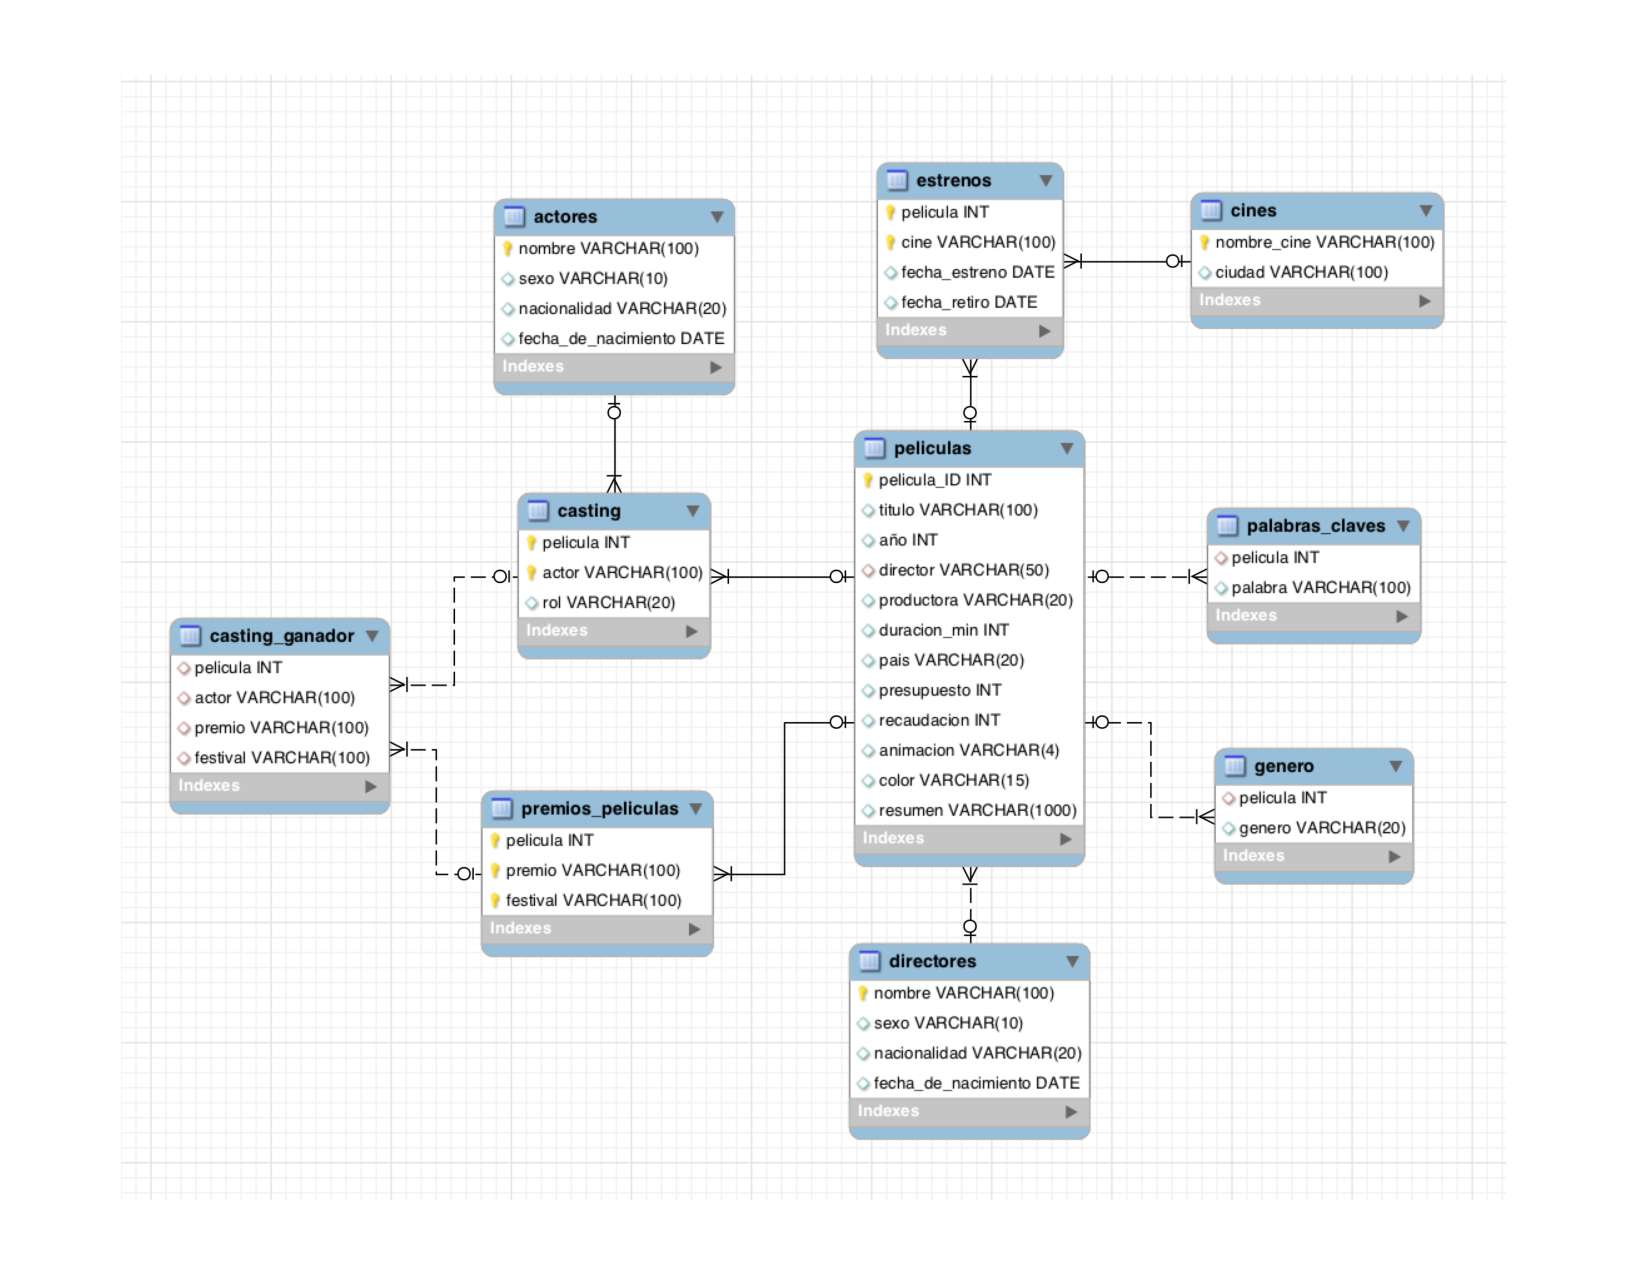
\includegraphics[width=\textwidth]{images/modelo todos.pdf}
%	\caption{Diagrama de cada una de las bases de datos}
%	\label{fig:diag}
%\end{figure}

\centering
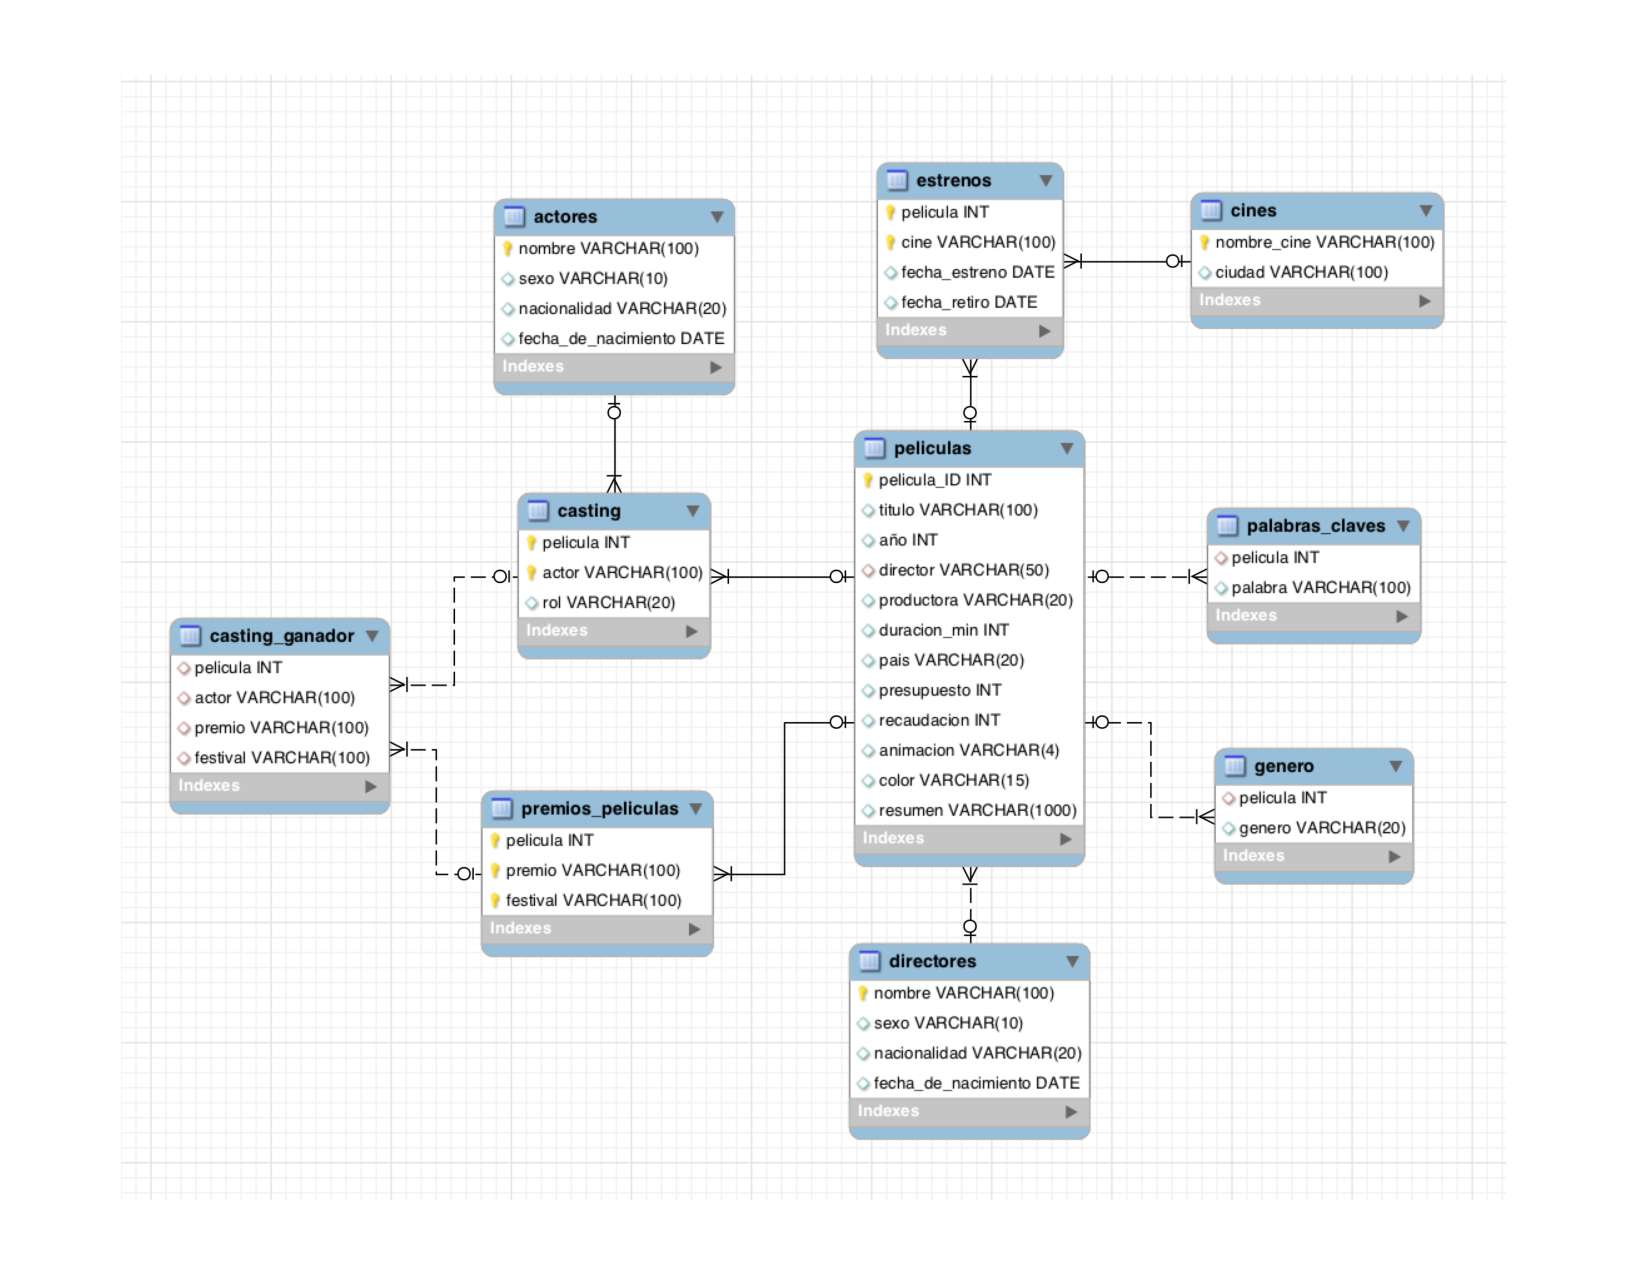
\includepdf[pages={1,2,3}]{images/modelo-todos.pdf}

\end{document}
